\documentclass{standalone}
\usepackage{tikz}

\begin{document}
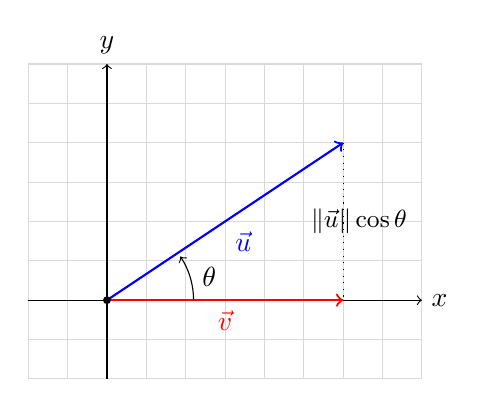
\begin{tikzpicture}
    % Draw a grid
    \draw[step=0.5,gray!30,thin] (-1,-1) grid (4,3);
    
    % Draw coordinate axes
    \draw[->] (-1,0) -- (4,0) node[right] {$x$};
    \draw[->] (0,-1) -- (0,3) node[above] {$y$};
    
    % Draw vectors
    \draw[->,thick,blue] (0,0) -- (3,2) node[midway,below right] {$\vec{u}$};
    \draw[->,thick,red] (0,0) -- (3,0) node[midway,below] {$\vec{v}$};
    
    % Draw angle between vectors
    \draw[->] (1.1,0) arc[start angle=0,end angle=33.69,radius=1cm];
    \node at (1.3,0.3) {$\theta$};
    
    % Draw dotted projections
    \draw[dotted] (3,2) -- (3,0);
    
    % Add labels
    \node at (3.2,1) {\small $\|\vec{u}\|\cos\theta$};
    
    % Enhance the origin
    \fill[black] (0,0) circle (0.05);
\end{tikzpicture}
\end{document}